\documentclass[12pt,]{article}
\usepackage{lmodern}
\usepackage{amssymb,amsmath}
\usepackage{ifxetex,ifluatex}
\usepackage{fixltx2e} % provides \textsubscript
\ifnum 0\ifxetex 1\fi\ifluatex 1\fi=0 % if pdftex
  \usepackage[T1]{fontenc}
  \usepackage[utf8]{inputenc}
\else % if luatex or xelatex
  \ifxetex
    \usepackage{mathspec}
    \usepackage{xltxtra,xunicode}
  \else
    \usepackage{fontspec}
  \fi
  \defaultfontfeatures{Mapping=tex-text,Scale=MatchLowercase}
  \newcommand{\euro}{€}
\fi
% use upquote if available, for straight quotes in verbatim environments
\IfFileExists{upquote.sty}{\usepackage{upquote}}{}
% use microtype if available
\IfFileExists{microtype.sty}{%
\usepackage{microtype}
\UseMicrotypeSet[protrusion]{basicmath} % disable protrusion for tt fonts
}{}
\usepackage[margin=1in]{geometry}
\ifxetex
  \usepackage[setpagesize=false, % page size defined by xetex
              unicode=false, % unicode breaks when used with xetex
              xetex]{hyperref}
\else
  \usepackage[unicode=true]{hyperref}
\fi
\hypersetup{breaklinks=true,
            bookmarks=true,
            pdfauthor={},
            pdftitle={Data Analysis with Topic Models for Communications Researchers},
            colorlinks=true,
            citecolor=blue,
            urlcolor=blue,
            linkcolor=magenta,
            pdfborder={0 0 0}}
\urlstyle{same}  % don't use monospace font for urls
\usepackage{graphicx,grffile}
\makeatletter
\def\maxwidth{\ifdim\Gin@nat@width>\linewidth\linewidth\else\Gin@nat@width\fi}
\def\maxheight{\ifdim\Gin@nat@height>\textheight\textheight\else\Gin@nat@height\fi}
\makeatother
% Scale images if necessary, so that they will not overflow the page
% margins by default, and it is still possible to overwrite the defaults
% using explicit options in \includegraphics[width, height, ...]{}
\setkeys{Gin}{width=\maxwidth,height=\maxheight,keepaspectratio}
\setlength{\parindent}{0pt}
\setlength{\parskip}{6pt plus 2pt minus 1pt}
\setlength{\emergencystretch}{3em}  % prevent overfull lines
\providecommand{\tightlist}{%
  \setlength{\itemsep}{0pt}\setlength{\parskip}{0pt}}
\setcounter{secnumdepth}{5}

%%% Use protect on footnotes to avoid problems with footnotes in titles
\let\rmarkdownfootnote\footnote%
\def\footnote{\protect\rmarkdownfootnote}

%%% Change title format to be more compact
\usepackage{titling}

% Create subtitle command for use in maketitle
\newcommand{\subtitle}[1]{
  \posttitle{
    \begin{center}\large#1\end{center}
    }
}

\setlength{\droptitle}{-2em}
  \title{Data Analysis with Topic Models for Communications Researchers}
  \pretitle{\vspace{\droptitle}\centering\huge}
  \posttitle{\par}
  \author{}
  \preauthor{}\postauthor{}
  \date{}
  \predate{}\postdate{}

\usepackage{setspace}
\doublespacing
\usepackage[nomarkers,figuresonly]{endfloat}
\usepackage[colorinlistoftodos]{todonotes}

% Redefines (sub)paragraphs to behave more like sections
\ifx\paragraph\undefined\else
\let\oldparagraph\paragraph
\renewcommand{\paragraph}[1]{\oldparagraph{#1}\mbox{}}
\fi
\ifx\subparagraph\undefined\else
\let\oldsubparagraph\subparagraph
\renewcommand{\subparagraph}[1]{\oldsubparagraph{#1}\mbox{}}
\fi

\begin{document}
\maketitle

\listoftodos

\section{Abstract}\label{abstract}

We present a non-technical introduction to data analysis with topic
models for communications researchers. We discuss important statistical
models and illustrate these methods with data from communications
scholarship. We complement our discussion with computer code (in the R
computing language) that implements these methods. We close with
thoughts about the future value of topic modeling to communications
researchers.
\todo[inline]{Do I want to emphasize data analysis more? I think so}

\section{Motivation}\label{motivation}

\todo[color=pink]{Can we write a scenario like that of Blei's 2012 article?}

We are in the big data era. Social media inundates us with status
updates and tweets, while bloggers share their views on current events.
These new media interact with more established media, such as print news
media, television, and radio. What do they have in common? One answer is
that they all can be viewed as data sources in which words - whether
written or spoken, tweeted or blogged - are the data.

Big data presents big opportunities for communications researchers.

We present a concise summary of a collection of machine learning
techniques that, together, are called ``topic modeling''. We discuss how
these methods may be used in communications research, and we apply topic
models to illustrative examples to demonstrate their value to
communications research questions.

\section{Overview}\label{overview}

The tremendous rise in computing speed and memory capacity, coupled with
the increasing avaialability of digitized texts, has enabled researchers
working at the interface of quantitative methods and social sciences to
treat written texts as data. While data analysis of documents is still
in its infancy, scientists nevertheless have made great progress towards
computational dissection and interpretation of texts. Among the most
foundational contributions is the development of probabilistic topic
models. We detail below, with limited use of statistical terminology,
how these methods work and why they may be useful in communications
research. We also provide an appendix with computer code (in the R
programming language) that implements these methods.

\todo[color = violet]{the above paragraphs are disjointed}

\section{What types of data analysis problems have others addressed with
topic
modeling?}\label{what-types-of-data-analysis-problems-have-others-addressed-with-topic-modeling}

\begin{itemize}
\tightlist
\item
  can we find several (3 or 4) motivating examples?
\end{itemize}

\begin{enumerate}
\def\labelenumi{\arabic{enumi}.}
\tightlist
\item
  genetics \& ancestral populations -- STRUCTURE paper 2000
\item
  political science 2010 paper\ldots{} on what??
\item
  what did John Dawson do?
\end{enumerate}

\section{What types of data?}\label{what-types-of-data}

\begin{enumerate}
\def\labelenumi{\arabic{enumi}.}
\tightlist
\item
  streaming\ldots{} what makes this interesting
\item
  hierarchical\ldots{} how?
\item
  Victorian Eyes
\end{enumerate}

\section{Box's Loop \& Data analysis}\label{boxs-loop-data-analysis}

\todo[inline, color=pink]{Need one or two figures here}

\missingfigure{Box's loop from 1976? Blei 2014?}

The perspective that guides our data analysis is based on ideas of the
University of Wisconsin-Madison statistician George Box and coworkers.
Blei (2014) extends the ideas of Box and colleagues to the specific case
of iterative refinement of topic models. Box (CITATION) articulated a
process of scientific inquiry and statistical collaboration in which
scientists put forth a hypothesis about the natural world, and, with
assistance from statisticians, design experiments to test the scientific
hypothesis. After statistical analysis of the experimental data, the
scientific hypothesis is refined, which leads to design and
implementation of another experiment, and the iterative process between
scientific hypothesis and experiment continues. Box also suggested
(CITATION) that a statistician, working in collaboration with
scientists, might use scientific questions as motivation to develop new
statistical methods in experimental design and data analysis. In this
sense, there is a second iterative loop by which a statistical
researcher develops novel methods because of their immediate need to
answer a scientific research question. Blei (2014) adapts these
iterative processes to the case of latent variable models, such as LDA
and related models. He argues that we view the use of a topic model for
a specific data analysis task as an iterative procedure in which one
proposes a simple topic model for the data analysis, fits the model,
interprets the results, and then, if needed, refines the topic model
with the goal of achieving data analysis results that are more
consistent with the research goals.

\section{Latent Dirichlet Allocation}\label{latent-dirichlet-allocation}

Blei, Ng, \& Jordan (2003) introduced a (generative) statistical model
called ``latent dirichlet allocation'' (LDA) in 2003. Although others
had described similar statistical models (Pritchard, Stephens, \&
Donnelly, 2000), Blei et al. (2003) first applied the statistical model
to text analysis. Researchers in a wide range of disciplines - including
genetics, linguistics, psychology, political science, and others - have
enthusiastically adopted LDA and related methods.

\subsection{What is the intuition behind the
model?}\label{what-is-the-intuition-behind-the-model}

As Blei (2012) writes, the key to understanding LDA is to recognize that
a given document - be it a research article, a novel, or a blog post -
exhibits multiple topics. Each topic, in turn, is, in a technical sense,
a distribution over words. For example, a topic related to evolution may
heavily weight the words ``evolution'', ``evolutionary'', ``biology'',
``phylogenetic'', and ``species''. In a given collection of documents,
which we term a ``corpus'' of documents, we assume that relatively few
topics - on the order of 10 to 50 for most analyses - are present.

\subsection{\texorpdfstring{In what sense is the model
`generative'?}{In what sense is the model generative?}}\label{in-what-sense-is-the-model-generative}

We say that LDA is a generative model because we specify a joint
probability distribution that allows generation of observed samples. In
a more precise manner, we specify a distribution over topics (again,
where topics are themselves distributions over words) that is shared by
the corpus. Each document can be viewed as a draw from this
distribution. The observed topic (distribution over words) tells us how
the words are distributed.

\section{LDA with statistical
terminology}\label{lda-with-statistical-terminology}

We can also describe LDA with more formal statistical terminology. We
let \(\beta_1, \beta_2, ..., \beta_K\) be the \(K\) topics, where each
\(\beta_k\) is a distribution over the vocabulary. Topic weights (or
proportions) we denote by \(\theta_d\) for the \(d^{th}\) document. We
let \(\theta_{d,k}\) be the topic proportion for topic \(k\) in document
\(d\). Topic assignments for the \(d^{th}\) document are \(z_d\), where
\(z_{d,n}\) is the topic assignment for the \(n^{th}\) word in the
\(d^{th}\) document. Observed words for the \(d^{th}\) document are
\(w_d\), where \(w_{d, n}\) is the \(n^{th}\) word for the \(d^{th}\)
document.

We then use the above notation to specify the joint distribution for all
variables in the model:

\[p(\beta_{1:K}, \theta_{1:D}, z_{1:D}, w_{1:D}) = \prod_{i = 1}^Kp(\beta_i)\prod_{d = 1}^Dp(\theta_d)\left( \prod_{n = 1}^N p(z_{d,n}|\theta_d)p(w_{d,n}|\beta_{1:K}, z_{d,n})\right)\]

The vertical bars in the last expressions denote conditional
probabilities. Note that the topic assignments \(z_{d,n}\) depend on the
document's topic proportions. Whatismore, the observed word \(w_{d,n}\)
has a distribution that depends on both the entire collection of topics,
\(\beta_{1:K}\), and the topic, \(z_{d,n}\), assigned to that word.

\section{Example of LDA with print
media}\label{example-of-lda-with-print-media}

An example may help to illustrate our point.

\begin{itemize}
\tightlist
\item
  which example to use here? NY Times
\end{itemize}

We analyzed

Blei \& Lafferty (2007) fitted a 100-topic model to 17,000 research
articles from the journal Science. They found that a 1996 article
``Seeking Life's Bare (Genetic) Necessities'' (Pennisi, 1996) exhibited
topics related to ``evolution'', ``genetics'', ``disease'', and
``computers''. \textbf{Would it be more sensible to use RT's Super Bowl
results here?}

\subsection{What is the model?}\label{what-is-the-model}

LDA models have a hiearchical structure in which words make up
documents, and a collection of documents is a corpus. The corpus is
assumed to have (unobserved) topics, or themes. The purposes of LDA,
then, are to discover the unobserved topics from the texts and to
characterize documents by the topics that they contain.

We distinguish generative models from discriminative models. A
generative model, such as LDA, is one in which we specify a joint
probability distribution for all variables (including those that are
unobserved) and, thus, enable the creation of observations. On the other
hand, a discriminative model relies on a conditional distribution and
doesn't permit generation of samples from the joint distribution.

\subsection{What are its assumptions?}\label{what-are-its-assumptions}

\subsection{What are its limitations?}\label{what-are-its-limitations}

The original LDA model However, LDA's flexibility and adaptability have
reduced the impact of its initial limitations. In the last decade,
researchers have devised extensions of LDA, such as ``dynamic LDA'',
that enable one to model topic evolution over time. Another extension of
LDA, which is known as ``correlated LDA'', accounts for correlations
among topics.

\section{Inference in topic models}\label{inference-in-topic-models}

Existing strategies for fitting topic models can be divided into two
classes: 1. variational Bayes methods and 2. sampling methods.
Variational Bayes methods try to approximate the posterior distribution
by maximizing a lower bound. In this sense, variational Bayes methods
approach topic model fitting from a computer science optimization
perspective. Alternatively, sampling methods, such as those based on
Markov chain monte carlo (MCMC) approaches, draw samples from (an
approximation to) the posterior distribution and estimate distributional
parameters by their empirical sample statistics.

Computational implementations of both classes of strategies are freely
available for the R statistical computing language. We include code to
use these free implementations in the appendix.

\section{Interpreting results of topic
modeling}\label{interpreting-results-of-topic-modeling}

Statistical inference for topic models yields estimates for topics
(i.e., distributions over words), assignments of words (within
documents) to topics, and weights of topics in each document.

The user must impose meaning on the topics. For instance, a topic may
put heavy weights on the words ``genetics'', ``gene'', ``regulation'',
``DNA'', ``transcription'', and ``RNA''. The data analyst needs to
identify the similarities among these words - namely, that they describe
concepts related to genetics and molecular biology. Fortunately, topic
modeling procedures often generate topics that can be summarized in one
or two words once the data analyst has inspected the most heavily
weighted terms (for a given topic).

\section{Visualizing topics}\label{visualizing-topics}

\begin{itemize}
\tightlist
\item
  LDAvis
\item
  wordcloud
\end{itemize}

Visualizing topic modeling results is an active area of research. We
present below strategies that involve static and interactive displays.

Word clouds are a widely used method for presenting topic modeling
results. Unfortunately, the standard approach requires a distinct word
cloud for each topic. For models with more than ten topics, manually
examining wordclouds becomes unwieldy. For a single topic, the default
method for creating a word cloud involves the identification of the most
heavily weighted words in the topic. The user may choose to assign font
sizes that are proportional to the weights of each word. One newly
developed method, which is implemented in the LDAvis R package, uses a
singular value decomposition of the fitted document-topic matrix to
calculate principal components. Each topic is then plotted in two
dimensions, where the axes represent the first two principal components.
The LDAvis R package enhances this second approach by making the figures
interactive with D3 javascript.

\section{\texorpdfstring{Results from NY Times ``Obama''
Analysis}{Results from NY Times Obama Analysis}}\label{results-from-ny-times-obama-analysis}

\begin{figure}
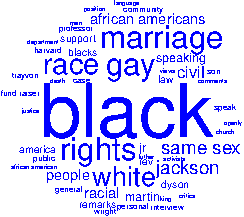
\includegraphics[width=\textwidth]{2016-03-17-obama_files/figure-latex/wordcloud-3.pdf}
\caption{Wordcloud for one topic from a 20-topic model. Larger font size corresponds to greater weight of that word in this topic.\label{fig:wc3}}
\end{figure}

We examine several wordclouds of topics derived from our analysis of 267
New York Times articles that contain the word ``Obama''. We notice in
Figure \ref{fig:wc3} words that relate to civil rights. Words that
emphasize race or sexual orientation feature prominently. It's possible
that if we were to fit a model with more topics, say 50, that race and
sexual orientation might occupy distinct topics.

\begin{figure}
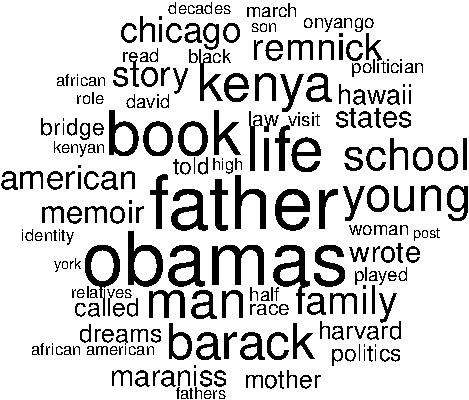
\includegraphics[width=\textwidth]{2016-03-17-obama_files/figure-latex/wordcloud-4.pdf}
\caption{Wordcloud for one topic from a 20-topic model. Larger font size corresponds to greater weight of that word in this topic.\label{fig:wc4}}
\end{figure}

Figure \ref{fig:wc4} contains words that deal with Barack Obama's
biography.

\begin{figure}
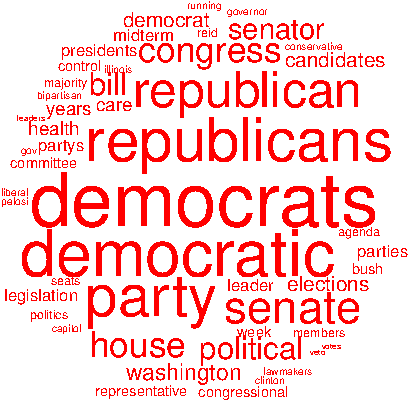
\includegraphics[width=\textwidth]{2016-03-17-obama_files/figure-latex/wordcloud-5.pdf}
\caption{Wordcloud for one topic from a 20-topic model. Larger font size corresponds to greater weight of that word in this topic.\label{fig:wc5}}
\end{figure}

Whatismore, Figure \ref{fig:wc5} highlights the use of political terms
in articles that contain the word ``Obama''.

\begin{figure}
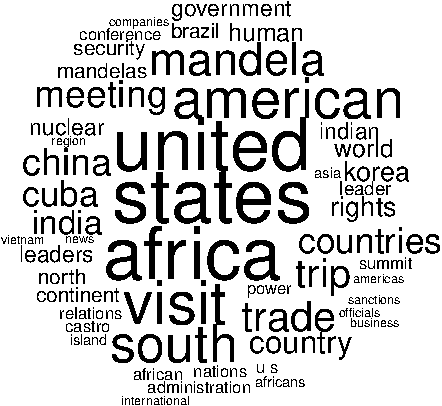
\includegraphics[width=\textwidth]{2016-03-17-obama_files/figure-latex/wordcloud-8.pdf}
\caption{Wordcloud for one topic from a 20-topic model. Larger font size corresponds to greater weight of that word in this topic.\label{fig:wc8}}
\end{figure}

International relations words make up the topic visualized in Figure
\ref{fig:wc8}.

\section{Discussion}\label{discussion}

\section{Future directions}\label{future-directions}

\section{Online resources}\label{online-resources}

David Mimno, a Cornell University scholar, curates an annotated
bibliography of topic modeling research(Mimno, 2016). His bibliography
is available at this url:
\url{http://mimno.infosci.cornell.edu/topics.html}

\section{Computational implementation of LDA with
R}\label{computational-implementation-of-lda-with-r}

We present below instructions and code for using LDA in the R
statistical computing language (R Core Team, 2015). \textbf{Ask Dhavan
about including code?} \textbf{Maybe as an appendix?}

\section*{References}\label{references}
\addcontentsline{toc}{section}{References}

\hypertarget{refs}{}
\hypertarget{ref-blei2012probabilistic}{}
Blei, D. M. (2012). Probabilistic topic models. \emph{Communications of
the ACM}, \emph{55}(4), 77--84.

\hypertarget{ref-blei2014build}{}
Blei, D. M. (2014). Build, compute, critique, repeat: Data analysis with
latent variable models. \emph{Annual Review of Statistics and Its
Application}, \emph{1}, 203--232.

\hypertarget{ref-blei2007correlated}{}
Blei, D. M., \& Lafferty, J. D. (2007). A correlated topic model of
science. \emph{The Annals of Applied Statistics}, 17--35.

\hypertarget{ref-blei2003latent}{}
Blei, D. M., Ng, A. Y., \& Jordan, M. I. (2003). Latent dirichlet
allocation. \emph{The Journal of Machine Learning Research}, \emph{3},
993--1022.

\hypertarget{ref-mimno2016topic}{}
Mimno, D. (2016). Topic modeling bibliography. Retrieved from
\url{http://mimno.infosci.cornell.edu/topics.html}

\hypertarget{ref-pennisi1996seeking}{}
Pennisi, E. (1996). Seeking life's bare (genetic) necessities.
\emph{Science}, \emph{272}(5265), 1098--1099.

\hypertarget{ref-pritchard2000inference}{}
Pritchard, J. K., Stephens, M., \& Donnelly, P. (2000). Inference of
population structure using multilocus genotype data. \emph{Genetics},
\emph{155}(2), 945--959.

\hypertarget{ref-r2015}{}
R Core Team. (2015). \emph{R: A language and environment for statistical
computing}. Vienna, Austria: R Foundation for Statistical Computing.
Retrieved from \url{https://www.R-project.org/}

\end{document}
